% !TEX root = ../paper.tex


% figure1
\begin{figure*}[htb] % cross-column image 
	\centering
	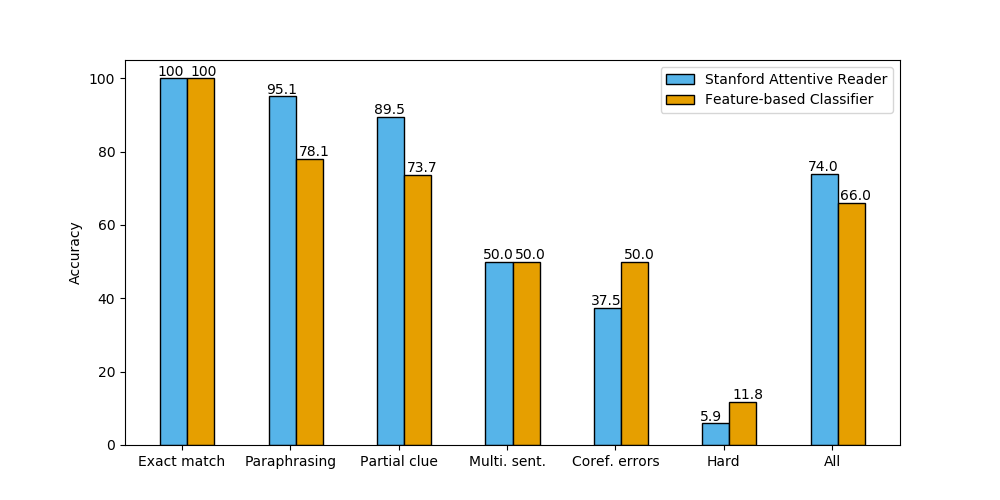
\includegraphics[scale=0.6]{img/cnn_analysis.png} 	% relative to paper.tex
	\caption{Differences in pre-training model architectures. BERT uses a bidirectional Transformer. OpenAI GPT uses a left-to-right Transformer. ELMo uses the concatenation of independently trained left-to-right and right- to-left LSTM to generate features for downstream tasks. Among three, only BERT representations are jointly conditioned on both left and right context in all layers.}
	\label{fig1}
\end{figure*}
	
% figure2
\begin{figure*}[htb] % cross-column image 
	\centering
	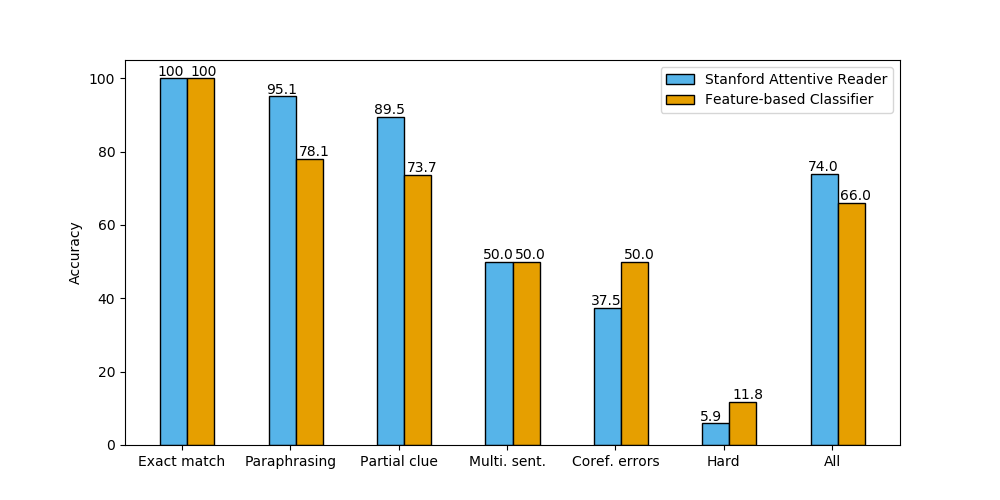
\includegraphics[scale=0.6]{img/cnn_analysis.png} 	% relative to paper.tex
	\caption{BERT input representation. The input embeddings is the sum of the token embeddings, the segmentation embeddings and the position embeddings.}
	\label{fig2}
\end{figure*}

\begin{figure*}[htb] % cross-column image 
	\centering
	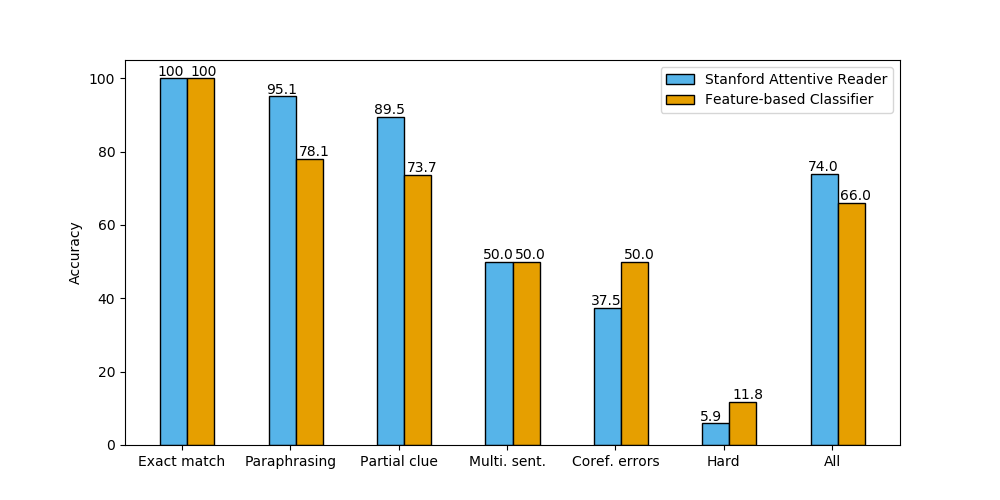
\includegraphics[scale=0.6]{img/cnn_analysis.png} 	% relative to paper.tex
	\caption{Our task specific models are formed by incorporating BERT with one additional output layer, so a minimal number of parameters need to be learned from scratch. Among the tasks, (a) and (b) are sequence-level tasks while (c) and (d) are token-level tasks. In the figure, E represents the input embedding, Ti represents the contextual representation of token i, [CLS] is the special symbol for classification output, and [SEP] is the special symbol to separate non-consecutive token sequences.}
	\label{fig3}
\end{figure*}
	
	
	
\section {BERT} \label{sec3}
We introduce BERT and its detailed implementation in this section. We first cover the model architecture and the input representation for BERT. We then introduce the pre-training tasks, the core innovation in this paper, in Section \ref{sec3.3}. The pre-training procedures, and fine-tuning procedures are detailed in Section \ref{sec3.4} and \ref{sec3.5}, respectively. Finally, the differences between BERT and OpenAI GPT are discussed in Section \ref{sec3.6}.

	\subsection {Model Architecture} \label{sec3.1}
	BERT's model architecture is a multi-layer bidirectional Transformer encoder based on the original implementation described in \citep{Ashish2017} and released in the \texttt{tensor2tensor} library \footnote{https://github.com/tensorflow/tensor2tensor}. Because the use of Transformers has become ubiquitous recently and our implementation is effectively identical to the original, we will omit an exhaustive background descriptioin of the model architecture and refer readers to \citet{Ashish2017} as well as excellent guides such as ``The Annotated Transformer.''\footnote{http://nlp.seas.harvard.edu/2018/04/03/attention.html}
	In this work, we denote the number of layers (i.e., Transformer blocks) as $L$, the hidden size as $H$, and the number of self-attention heads as $A$. In all cases we set the feed-forward/filter size to be $4H$, i.e., 3072 for the $H = 768$ and 4096 for the $H = 1024$. We primarily report results on two model sizes:
	\begin{itemize}
		\item \bm{${\rm BERT_{BASE}}$} L=12, H=768, A=12, Total Parameters=110M % bold and rectified underline
		\item \bm{${\rm BERT_{LARGE}}$}: L=24, H=1024, A=16, Total Parameters=340M
	\end{itemize}
	$\rm BERT_{BASE}$ was chosen to have an identical model size as OpenAI GPT for comparison purposes. Critically, however, the BERT Transformer uses bidirectional self-attention, while the GPT Transformer uses constrained self-attention where every token can only attend to context to its left. We not that in the literature the bidirectional Transformer is often referred to as a ``Transformer encoder'' while the left-context-only version is referred to as a ``Transformer decoder'' since it can be used for text generation. The comparisons between BERT, OpenAI GPT and ELMo are shown visually in Figure \ref{fig1}.
	
	\subsection {Input Representation} \label{sec3.2}
	Our input representation is able to unambiguously represent both a single text sentence or a pair of text sentences (e.g., [Question, Answer]) in one token sequence \footnote{Throughout this work, a “sentence” can be an arbitrary span of contiguous text, rather than an actual linguistic sen- tence. A “sequence” refers to the input token sequence to BERT, which may be a single sentence or two sentences packed together.}. For a give token, its input representation is constructed by summing the corresponding token, segment and position embeddings. A visual representation of our input representation is give in Figure \ref{fig2}.
	
	The specifics are:
	\begin{itemize}
		\item We use WordPiece embeddings \citep{Yonghui2016} with a 30000 token vocabulary. We denote split word pieces with \#\#.
		\item We use learned positional embeddings with supported sequence lengths up to 512 tokens.
		\item The first token of every sequence is always the special classification embedding ([CLS). The final hidden state (i.e., output of Transformer) corresponding to this token is used as the aggregate sequence representation for classification tasks. For non-classification tasks, this vector is ignored.
		\item Sentence pairs are packed together into a single sequence. We differentiate the sentences in two ways. First, we separate them with a special token ([SEP]). Second, we add a learned sentence $A$ embedding to every token of the first sentence and a sentence $B$ embedding to every token of the second sentence.
		\item For single-sentence inputs we only use the sentence $A$ embeddings.
	\end{itemize}
	
	\subsection {Pre-training Tasks} \label{sec3.3}
	Unlike \citet{Matthew2018} and \citet{Alec2018}, we do not use traditional left-to-right or right-to-left language models to pre-train BERT. Instead, we pre-train BERT using two novel unsupervised prediction tasks, described in this section.
	
		\subsubsection{Task \#1: Masked LM} \label{sec3.3.1}
		Intuitively, it is reasonable to believe that a deep bidirectional model is strictly more powerful than either a left-to-right model or the shallow concatenation of a left-to-right and right-to-left model. Unfortunately, standard conditional language models can only be trained left-to-right \emph{or} right-to-left, since bidirectional conditioning would allow each word to indirectly ``see itself'' in a multi-layered context.
		
		In order to train a deep bidirectional representation, we take a straightforward approach of masking some percentage of the input tokens at random, and then predicting only those masked tokens. We refer to this procedure as a ``masked LM''(MLM), although it is often referred to as a \emph{Cloze} task in the literature \citep{Wilson1953}. In this case, the final hidden vectors corresponding to the mask tokens are fed into an output softmax over the vocabulary, as in a standard LM. In all of our experiments, we mask 15\% of all WordPiece tokens in each sequence at random. In contrast to denoising auto-encoders \citep{Pascal2008}, we only predict the masked words rather than reconstructing the entire input.
		
		Although this does allow us to obtain a bidirectional pre-trained model, there are two downsides to such an approach. The first is that we are creating a mismatch between pre-training and fine-tuning, since the {\fontfamily{pcr}\selectfont[MASK]} token is never seen during fine-tuning. To mitigate this, we do not always replace ``masked'' words with the actual {\fontfamily{pcr}\selectfont[MASK]} token. Instead, the training data generator chooses 15\% of tokens at random, e.g., in the sentence {\small{\fontfamily{pcr}\selectfont my dog is hairy}} it chooses {\small{\fontfamily{pcr}\selectfont hairy}}. It then performs the following procedure:
		\begin{itemize}
			\item Rather than \emph{always} replacing the chosen words with {\fontfamily{pcr}\selectfont[MASK]}, the data generator will do the following: 
			\item 80\% of the time: Replace the word with {\fontfamily{pcr}\selectfont[MASK]} token, e.g., {\small{\fontfamily{pcr}\selectfont my dog is hairy -> my dog is [MASK]}} 
			\item 10\% of the time: Replace the word with a random word, e.g., {\small{\fontfamily{qcr}\selectfont my dog is hairy -> my dog is apple}} 
			\item 10\% of the time: Keep the word unchanged, e.g., {\small{\fontfamily{pcr}\selectfont my dog is hairy -> my dog is hairy}}. The purpose of this is to bias the representation towards the actual observed word. 
		\end{itemize}
		
		The Transformer encoder does not know which words it will be asked to predict or which have been replaced by random words, so it is forced to keep a distributional contextual representation of \emph{every} input token. Additionally, because random replacement only occurs for 1.5\% of all tokens (i.e., 10\% of 15\%), this does not seem to harm the model's language understanding capability.
		
		The second downside of using an MLM is that only 15\% of tokens are predicted in each batch, which suggests that more pre-training steps may be required for the model to coverage. In Section \ref{sec5.3} we demonstrate that MLM does converge marginally slower than a left-to-right model (which predicts every token), but the empirical improvements of the MLM model far outweigh the increased training cost.
		
		\subsubsection{Task \#2: Next Sentence Prediction} \label{sec3.3.2}
		Many important downstream tasks such as Question Answering (QA) and Natural Language Inference (NLI) are based on understanding the \emph{relationship} between two text sentences, which is not directly captured by language modeling. In order to train a model that understands sentence relationship, we pre-train a binarized \emph{next sentence prediction} task that can be trivially generated from any monolingual corpus. Specifically, when choosing the sentences {\fontfamily{pcr}\selectfont A} and {\fontfamily{pcr}\selectfont B} for each pre-training example, 50\% of the time {\fontfamily{pcr}\selectfont B} is the actual next sentence that follows {\fontfamily{pcr}\selectfont A}, and 50\% of the time it is a random sentence from the corpus. For example:
		
		\begin{table}[h]
		\begin{tabular}{ccl}
		Input & = & \scriptsize{{\fontfamily{pcr}\selectfont [CLS] the man went to [MASK] store [SEP]}} \\
		&& \scriptsize{{\fontfamily{pcr}\selectfont he bought a gallon [MASK] milk [SEP]}} \\
		Label & = & \scriptsize{{\fontfamily{pcr}\selectfont IsNext }} \\
		&& \\
		Input & = & \scriptsize{{\fontfamily{pcr}\selectfont [CLS] the man [MASK] to the store [SEP]}} \\
		&& \scriptsize{{\fontfamily{pcr}\selectfont penguin [MASK] are flight \#\#less birds [SEP]}} \\
		Label & = & \scriptsize{{\fontfamily{pcr}\selectfont NotNext }} \\
		\end{tabular}
		\end{table}
		
		We choose the {\fontfamily{pcr}\selectfont NotNext} sentences completely at random, and the final pre-trained model achieves 97\%-98\% accuracy at this task. Despite its simplicity, we demonstrate in Section \ref{sec5.1} that pre-training towards this task is very beneficial to both QA and NLI.
		
	\subsection {Pre-training Procedure} \label{sec3.4}
	The pre-training procedure largely follows the existing literature on language model pre-training. 
	
	For the pre-training corpus we use the concatenation of BooksCorpus (800M words) \citep{Yukun2015} and English Wikipedia (2500M words). For Wikipedia we extract only the text passages and ignore lists, tables, and headers. It is critical to use a document-level corpus rather than a shuffled sentence-level corpus such as the Billion Word Benchmark \citep{Ciprian2013} in order to extract long contiguous sequences. 
	
	To generate each training input sequence, we sample two spans of text from the corpus, which we refer to as ``sentences'' even though they are typically much longer than single sentences (but can be shorter also). The first sentence receives the {\fontfamily{pcr}\selectfont A} embedding and the second receives the {\fontfamily{pcr}\selectfont B} embedding. 50\% of the time {\fontfamily{pcr}\selectfont B} is the actual next sentence that follows {\fontfamily{pcr}\selectfont A} and 50\% of the time it is a random sentence, which is done for the ``next sentence prediction'' task. They are sampled such that the combined length is $\le$ 512 tokens. The LM masking is applied after WordPiece tokenization with a uniform masking rate of 15\%, and no special consideration given to partial word pieces. 
	
	We train with batch size of 256 sequences (256 sequences * 512 tokens = 128000 tokens/batch) for 1000000 steps, which is approximately 40 epochs over the 3.3 billion word corpus. We use Adam with learning rate of 1e-4, $\beta_1 = 0.9$, $\beta_2 = 0.999$, L2 weight decay of 0.01, learning rate warmup over the first 10000 steps, and linear decay of the learning rate. We use a dropout probability of 0.1 on all layers. We use a {\fontfamily{pcr}\selectfont gelu} activation \citep{Dan2016} rather than the standard {\fontfamily{pcr}\selectfont relue}, following OpenAI GPT. The training loss is the sum of the mean masked LM likelihood and mean next sentence prediction likelihood.
	
	Training of $\rm BERT_{BASE}$ was performed on 4 Cloud TPUs in Pod configuration (16 TPU chips total)\footnote{https://cloudplatform.googleblog.com/2018/06/Cloud-TPU-now-offers-preemptible-pricing-and-global- availability.html}. Training of $\rm BERT_LARGE$ was performed on 16 Cloud TPUs (64 TPU chips total). Each pre-training took 4 days to complete.
	
	\subsection {Fine-tuning Procedure} \label{sec3.5}
	For sequence-level classification tasks, BERT fine-tuning is straightforward. In order to obtain a fixed-dimensional pooled representation of the input sequence, we take the final hidden state (i.e., the output of the Transformer) fo the first token in the input, which by construction corresponds to the special {\fontfamily{pcr}\selectfont [CLS]} word embedding. We denote this vector as $C \in \R^H$. The only new parameters added during fine-tuning are for a classification layer $W \in \R^{K*H}$, where $K$ is the number of classifier labels. The label probabilities $P \in \R^K$ are computed with a standard softmax, $P=softmax(CW^T)$. All of the parameters of BERT and $W$ are fine-tuned jointly to maximize the log-probability of the correct label. For span-level and token-level prediction tasks, the above procedure must be modified slightly in a task-specific manner. Details are given in the corresponding subsection of Section \ref{sec4}.
	
	For fine-tuning, most model hyperparameters are the same as in pre-training, with the exception of the batch size, learning rate, and number of training epochs. The dropout probability was always kept at 0.1. The optimal hyperparameter values are task-specific, but we found the following range of possible values to work well across all tasks:
	
		\begin{itemize}
			\item \textbf{Batch size}: 16, 32
			\item \textbf{Learning rate (Adam)}: 53-5, 3e-5, 2e-5
			\item \textbf{Number of epochs}: 3, 4
		\end{itemize}
		
	We also observed that large data sets (e.g., 100k+ labeled training examples) were far less sensitive to hyperparameter choice than small data sets. Fine-tuning is typically very fast, so it is reasonable to simply run an exhaustive search over the above parameters and choose the model that performs best on the development set.
	
	\subsection {Comparison of BERT and OpenAI GPT} \label{sec3.6}
	The most comparable existing pre-training method to BERT is OpenAI GPT, which trains a left-to-right Transformer LM on a large text corpus. In fact, many of the design decisions in BERT were intentionally chosen to be as close to GPT as possible so that the two methods could be minimally compared. The core argument of this work is that the two novel pre-training tasks  presented in Section \ref{sec3.3} account for the majority of the empirical improvements, but we do not that there are several other differences between how BERT and GPT were trained:
	
		\begin{itemize}
			\item GPT is trained on the BooksCorpus (800M words); BERT is trained on the BooksCorpus (800M words) and Wikipedia (2500M words).
			\item GPT uses a sentence separator ([SEP]) and classifier token ([CLS]) which are only introduced at fine-tuning time; BERT learns [SEP], [CLS] and sentence A/B emeddings during pre-training.
			\item GPT was trained for 1M steps with a batch size of 32000 words; BERT was trained for 1M steps with a batch size of 128000 words.
			\item GPT used the same learning rate of 5e-5 for all fine-tuning experiments; BERT chooses a task-specific fine-tuning learning rate which performs the best on the development set.
		\end{itemize}
		
	To isolate the effect of these differences, we perform ablation experiments in Section \ref{sec5.1} which demonstrates that the majority of the improvements are in fact coming form the new pre-training tasks.
	
	
	
	
	